\documentclass[12pt]{article}
\usepackage{fullpage, amsmath, amssymb, amsthm, amscd, setspace, bm, graphicx, indentfirst, multirow, tikz, enumerate}
\usepackage{adjustbox,amsfonts,array,graphicx,booktabs,tabularx,multirow,multicol,stmaryrd, tabu}
\usepackage[utf8]{inputenc}
\usetikzlibrary{arrows.meta}
\title{Math 412, Fall 2023 -- Homework 5}
\date{}
\setlength{\parskip}{0.5cm}
\setlength{\parindent}{0cm}

\newtheorem{theorem}{Theorem}[section]
\newtheorem{definition}[theorem]{Definition}
\newtheorem{lemma}[theorem]{Lemma}
\newtheorem{proposition}[theorem]{Proposition}
\newtheorem{corollary}[theorem]{Corollary}
\newtheorem{remark}[theorem]{Remark}
\newtheorem{example}[theorem]{Example}

\newcommand{\Z}{\mathbb{Z}}
\newcommand{\R}{\mathbb{R}}
\newcommand{\Q}{\mathbb{Q}}
\newcommand{\C}{\mathbb{C}}
\newcommand{\ba}{\overline}
\newcommand{\Hom}{\text{Hom}}
\newcommand{\End}{\text{End}}
\newcommand{\wt}[1]{\text{wt}({#1})}
\newcommand{\sgwt}[1]{\text{sgwt}({#1})}
\begin{document} \maketitle
\vspace{-80pt}

\textbf{Due:} Wednesday, October 4th, at 9:00AM via Gradescope

\textbf{Instructions:} Students taking the course for three credit hours (undergraduates, most graduate
students) should complete \textbf{all three} of the following problems. Graduate students
taking the course for four credits should contact the instructor. The first problem will count double in the grading. Problems that use the word ``describe”, ``determine”, ``show", or ``prove" require proof for all claims.

\begin{enumerate}

\item[1.] In this problem, we will prove the weighted Matrix Tree Theorem by using the unweighted analogue. Recall the definitions from class of the tree sum $\tau(G)$ and the Laplacian $L^i(G)$ for weighted graphs.

\begin{enumerate}
    \item[(a)] Let $f(x_1,\ldots,x_k):\R^k\to \R$ and $g(x_1,\ldots,x_k):\R^k\to\R$ be polynomials in $k$-variables $x_1,\ldots, x_k$. If for all $k$-tuples $(a_1,\ldots,a_k)$ of positive integers, we have $f(a_1,\ldots,a_k) = g(a_1,\ldots,a_k)$, prove that $f$ and $g$ are equal for \emph{any} inputs. \emph{[Hint: think of $f$ and $g$ as polynomials only in $x_k$, and consider $f-g$. Use induction on $k$.]}
    
    \item[(b)] Let $G$ be a weighted loopless graph with positive integer weights. Using the (unweighted) Matrix Tree Theorem, prove that for any $i$, $\tau(G) = \det L^i(G)$. \emph{[Hint: consider the unweighted graph $G'$ formed from $G$ by taking each edge $e$ of $G$ with weight $w$ and, and letting $G'$ have $w$ edges with the same endpoints as $e$.]}

    \item[(c)] Combine (a) and (b) to prove the weighted Matrix Tree Theorem: if $G$ is a weighted loopless graph with any weights, then for any $i$, $\tau(G) = \det L^i(G)$. \emph{[Hint: think of the edge weights as variables, and explain why part (a) holds.]}

\end{enumerate}

\item[2.] Let $D$ be a weakly-connected weighted loopless digraph with underlying graph $G$.

For any walk $W$ in $G$, define the signed weight of $W$ to be \[\sgwt{W} = \sum_{e\in E(W)}\pm \wt{e},\] where the sign on $\wt{e}$ is positive if and only if we traverse $e$ from tail to head.

Fix a vertex $v\in V(G)$. Prove that the following conditions are equivalent.

\begin{enumerate}
    \item[(K2)] For any closed walk $C$ in $G$, $\sgwt{C}=0$.
    \item [(K2')] There exists a unique function $U:V(G)\to \R$ such that $U(v)=0$ and for all $e\in E(D)$, \[\wt{e} = U(\text{head of $e$}) - U(\text{tail of $e$}).\]
\end{enumerate}

\emph{[Hint: if $U(v)=0$ and $W$ is a walk from $v$ to $u$, what must be true about $U(u)$?]}

\item[3.] For the following (unweighted) graph $G$, compute $\tau(G)$, $L(G)$, $\det L^1(G)$ and $\det L^2(G)$, and thus confirm the Matrix Tree Theorem for this example.

\begin{center}
\scalebox{0.7}{
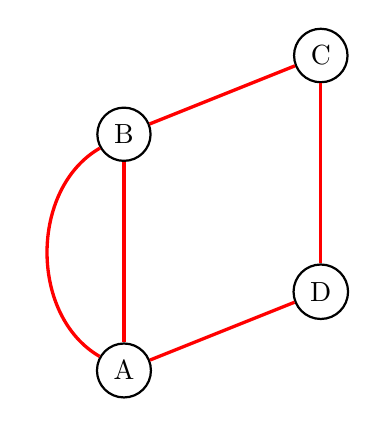
\begin{tikzpicture}
\begin{scope}[every node/.style={circle,thick,draw}]
    \node (A) at (0,0) {A};
    \node (B) at (0,3) {B};
    \node (C) at (2.5,4) {C};
    \node (D) at (2.5,1) {D};
\end{scope}

\begin{scope}[>={Stealth[black]},
              every node/.style={fill=white,circle},
              every edge/.style={draw=red,very thick}]
    \path [-] (A) edge (B);
    \path [-] (B) edge (C);
    \path [-] (A) edge (D);
    \path [-] (D) edge (C);
    \path [-] (B) edge[bend right=60] (A); 
\end{scope}
\end{tikzpicture}}
\end{center}


\end{enumerate}

\end{document}
